% LTex: language=pl
\section{Iteracje projektu oraz zmiany stanu wiedzy i wymagań}
Wymagania dotyczące docelowego systemu były pozyskiwane z poniższych źródeł:
\begin{itemize}
    \item Klient -- Osoba dobrze zaznajomiona z funkcjami systemu, posiadająca powierzchowną wiedzę na temat jego implementacji oraz będąca w posiadaniu dostępu do serwera, na którym zostanie uruchomione docelowe rozwiązanie. Jest głównym źródłem wymagań funkcjonalnych systemu.
    \item Administrator STOS -- Osoba znająca działanie systemu, potrafiąca uruchomić system i rozwiązać istniejące problemy.
    \item Studenci -- Bezpośredni użytkownicy systemu. Wymagania były zbierane poprzez ankiety, nieformalne rozmowy oraz doświadczenia autorów pracy.
    \item System STOS -- Nieożywione źródło wymagań. Jest to istniejąca implementacja systemu, działająca na serwerach katedry algorytmów i modelowania systemów. Docelowe środowisko powinno  integrować części komponentów tego systemu, dostosować się do interfejsów komunikacyjnych i odzwierciedlać funkcjonalności obecnych modułów.
\end{itemize}
Ze względu na uzależnienie platformy od odpowiedniej struktury systemu, ochronę algorytmu oceny oraz konieczność uzyskania zgody na publikację kodu przez jego autora, informacje o systemie były przekazywane dla naszego zespołu w sposób iteracyjny.
\newline \indent W pierwszej iteracji, datowanej na marzec 2024 roku, uzyskaliśmy informacje dotyczące istniejących problemów i ogólnego obrazu komponentów oraz ich roli. Ponieważ nie posiadaliśmy informacji na temat szczegółowego działania systemu, protokołów komunikacyjnych i środowiska docelowego, postanowiliśmy utworzyć przykładową wersję systemu, projektowaną z myślą o dynamicznie zmieniających się wymaganiach. Utworzony prototyp posiadał atrapę modułu oceniającego, serwisy Elasticsearch i Graylog pozwalające na gromadzenie i analizę logów, system zarządzający i gromadzący pliki oraz moduły pobierające, przekazujące i wykonujące pliki programów przesłanych przez studentów. Ze względu na szereg zalet konteneryzacji, wszystkie komponenty działały jako kontenery platformy Docker, zarządzane przez orkiestrator Kubernetes. Komunikacja pomiędzy serwisami odbywała się przez protokół http oraz kolejkę wiadomości RabbitMQ \cite{rabbit}. By zbadać trudność implementacji, możliwość integracji zewnętrznych systemów oraz wydajność różnych technologii, komponenty zostały zaimplementowane w językach Java, Golang, Python oraz Rust. W celu zachowania spójnego formatu wiadomości i ich poprawnego przesyłania oraz odczytania zastosowano mechanizm serializacji Protobuf \cite{protobuf}, opracowany i utrzymywany przez firmę Google. Każdy z komponentów przesyłał logi do platformy Elasticstack. Proponowane rozwiązanie działa w pięciu krokach:
\newline \indent 1. Komponent Task Poller pobiera zadanie z kolejki istniejącego komponentu STOS, który przechowuje pliki zadań przesłanych przez studenta. Z racji braku wiedzy o interfejsie komunikacji, założyliśmy komunikację przez protokół HTTP, który przesyła zestaw plików potrzebnych do kompilacji i oceny. Zadania tymczasowo były atrapami, a przesłane pliki nie uwzględniały pozostałych plików wymaganych w ocenie, takich jak oczekiwany rezultat.
\newline \indent 2. W kolejnym kroku zadania umieszczane są w kolejce. Największą zaletą stosowania tego komponentu, jest możliwość zredukowania czasu wykonywania logiki aplikacji, poprzez możliwość delegowania poszczególnych operacji do różnych serwisów, co w przypadku braku wiedzy o systemie, umożliwiało prostsze skalowanie architektury. Decyzja o użyciu tej kolejki zamiast jej równie popularnej, alternatywnej kolejki wiadomości Kafka, jest mechanizm niezawodnego przesłania wiadomości do konsumenta. Do komunikacji używany jest protokół AMQP.
\newline \indent 3. Komponent Worker, który jest subskrybentem kolejki, otrzymuje zadanie do wykonania. Komponent docelowo miał realizować funkcje kompilacji i oceny rozwiązania studentów. By zwiększyć niezawodność, pliki aktualnie ocenianego zadania, były umieszczane w kolejce. Serwis był uruchamiany jako kontener działający na platformie Docker.
\newline \indent 4. Na podstawie otrzymanych plików z wynikami oraz oczekiwanym rezultatem, dokonywana jest ocena.
\newline \indent 5. Rezultat zadania jest przesyłany do serwisu STOS poprzez protokół HTTP.
\begin{figure}[!h]
	\begin{center}
		\resizebox{1.0\textwidth}{!} {
			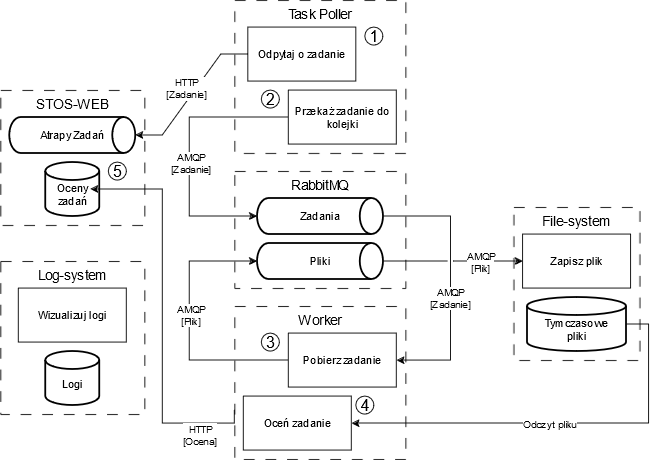
\includegraphics{img/1/i1_arch.png}
		}
		\caption[Architektura po pierwszej iteracji]{Diagram przedstawiający wysokopoziomową architekturę systemu, z uwzględnieniem komponentów, ich głównych funkcji oraz sposobu komunikacji w pierwszej iteracji projektu. Źródło własne.}
	\end{center}
\end{figure}
\newline \indent Druga iteracja projektu odbyła się w maju 2024 roku. Otrzymaliśmy wtedy informacje na temat szczegółowego działania komponentów w systemie oraz sekwencji operacji wykonywanych podczas procesu oceny zadania studenta. Zaznajomienie z komponentami pozwoliło nam na rozbudowę rozwiązania o mechanizm pamięci podręcznej. Kluczową otrzymaną informacją, był fakt działania modułu kompilującego w kontenerze na platformie Docker. W poprzedniej architekturze założyliśmy działanie całej strony serwerowej jako osobne serwisy uruchomione na tej samej maszynie wirtualnej, które w ramach docelowego systemu chcieliśmy przenieść do kontenera z naszym rozwiązaniem. Biorąc pod uwagę ścisłe powiązanie komponentów systemu i nowo otrzymaną informację, oznaczałoby uruchomienie zagnieżdżonego kontenera z modułem kompilującym w kontenerze z naszym rozwiązaniem. Znacząco podniosłoby to poziom skomplikowania, zarządzania systemem oraz detekcji awarii systemu. Opracowane rozwiązanie działało w dziewięciu krokach:
\newline \indent 1. Analogicznie do działania w pierwszej iteracji, komponent Task Poller pobiera zadanie z serwisu STOS. Ze względu na rezygnacje z kolejki RabbitMQ, pliki były zapisywane w pamięci.
\newline \indent 2. Komponent Task Poller zlecał ocenę otrzymanego zadania.
\newline \indent 3. Komponent Dispatcher pobierał odpowiednie pliki z pamięci cache. W przypadku ich braku były one pobierane z komponentu Task Poller. Zapewniało to przyspieszenie działania, w przypadku kompilacji rozwiązań używających tych samych plików z oczekiwanymi rezultatami.
\newline \indent 4. Uruchamiany był kolektor logów. Gromadził on wiadomości przesyłane na standardowe wyjście przez kontenery oceniające.
\newline \indent 5. W kolejnym kroku uruchomiony zostaje kontener kompilujący i oceniający rozwiązanie. Oprócz wydawania komendy uruchomienia przekazywał on też wymagane pliki.
\newline \indent 6. Zadanie jest kompilowane.
\newline \indent 7. Po pomyślnej kompilacji rozwiązanie jest uruchamiane i porównywane z oczekiwanym rezultatem. Po zakończeniu procesu, na standardowe wyjście przesyłany jest sygnał zakończenia.
\newline \indent 8. Gdy komponent Log-Harvester odczytał sygnał zakończenia procesu, przesyłał zgromadzone logi do serwisu Log-System poprzez protokół HTTP, które mogły zostać przetworzone.
\newline \indent 9. Przed emitowaniem sygnału wyjściowego, komponent Worker przesyłał ocenę do serwisu STOS.
\begin{figure}[!h]
	\begin{center}
		\resizebox{1.0\textwidth}{!} {
			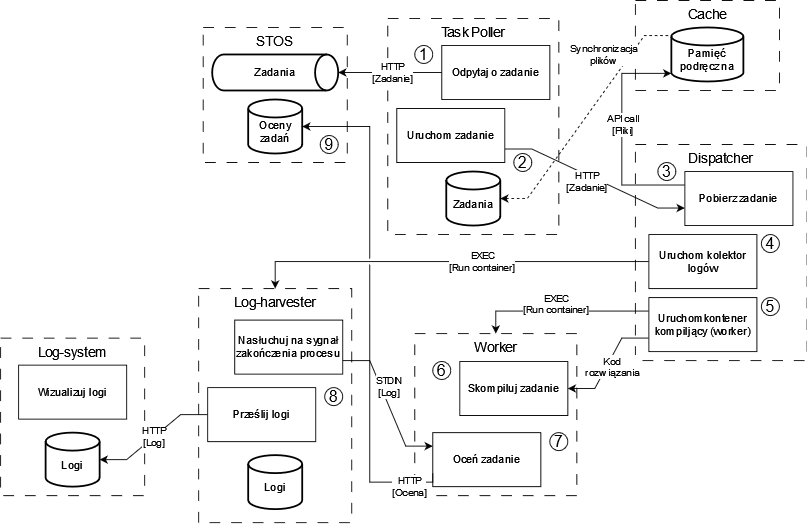
\includegraphics{img/1/i2_arch.png}
		}
		\caption[Architektura po drugiej iteracji]{Diagram przedstawiający wysokopoziomową architekturę systemu, z uwzględnieniem komponentów, ich głównych funkcji oraz sposobu komunikacji w drugiej iteracji projektu. Źródło własne.}
	\end{center}
\end{figure}
\newline \indent W trzeciej iteracji projektu, która odbyła się w czerwcu 2024 roku, zostały szczegółowo wyjaśnione sposoby komunikacji między komponentami. Zdecydowaliśmy się na zmianę architektury systemu, w której pozostawiliśmy moduł kompilujący w dotychczasowej formie, z dodatkiem funkcji powiadamiania o zakończonej pracy. Utworzyliśmy serwis zarządzający instancjami tych kontenerów oraz serwis pobierający i przekazujący zadania. Całość będzie umieszczona na nadzorcy pierwszego stopnia, który jest trzecią alternatywą dla maszyn wirtualnych i kontenerów. Stworzony system składał się z jednej aplikacji, co zwalniało konieczność implementacji protokołów komunikacji. Komponenty zapisywały zdarzenia do pliku z logami, odczytywany przez serwis Filebeat, który przesyłał je do serwera logów. Działanie systemu składa się z sześciu kroków:
\newline \indent 1. Komponent Manager pobiera zadanie przez protokół HTTP.
\newline \indent 2. Pobrane pliki zostały zapisywane w odpowiednim katalogu na serwerze. Do komponentu Scheduler, została przesłana komenda zlecająca kompilację. Dane są umieszczane w kolejce zadań oczekujących na obsługę.
\newline \indent 3. Gdy istnieje dostępny kontener, który może dokonać obsługi, zadanie jest do niego przesyłane. Zakładany jest brak konieczności uruchamiania kontenera, ponieważ powinien on działać w tle.
\newline \indent 4. Zadanie jest kompilowane i oceniane.
\newline \indent 5. Do komponentu Manager przesyłana jest informacja o ocenie.
\newline \indent 6. Manager, który jest pośrednikiem w komunikacji z serwerem STOS, po otrzymaniu wiadomości z oceną, przekazuje ją dalej.
\begin{figure}[!h]
	\begin{center}
		\resizebox{1.0\textwidth}{!} {
			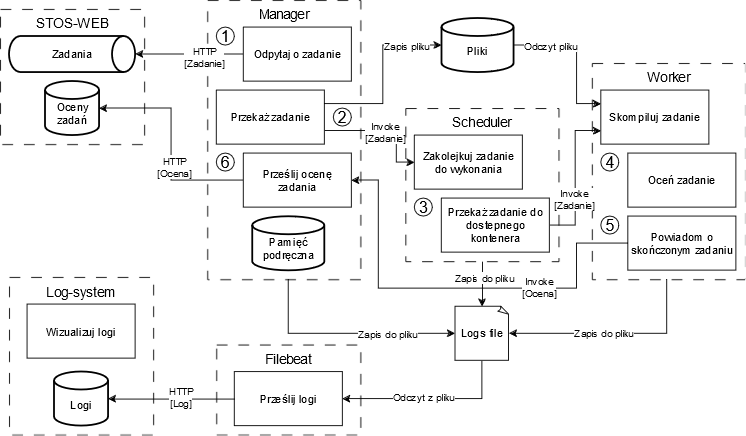
\includegraphics{img/1/i3_arch.png}
		}
		\caption[Architektura po trzeciej iteracji]{Diagram przedstawiający wysokopoziomową architekturę systemu, z uwzględnieniem komponentów, ich głównych funkcji oraz sposobu komunikacji w trzeciej iteracji projektu. Źródło własne.}
	\end{center}
\end{figure}
\newline \indent Czwarta iteracja odbyła się we wrześniu 2024 roku. Otrzymaliśmy wtedy informacje na temat docelowego systemu, na którym zostanie uruchomione tworzone rozwiązanie. Zostały również przekazane instrukcje do jego połączenia. Postanowiliśmy uruchomić i skonfigurować maszyny nadzorcy na serwerze. Skutkiem było uruchomienie środowisk deweloperskich, produkcyjnych oraz serwera logów. Sposób zarządzania został opisany w instrukcji, a poświadczenia zostały przekazane klientowi. Z racji nieuzależniania naszego rozwiązania od konkretnego systemu, nie wiązało się to ze zmianą architektury i implementacji. 
\newline \indent Ostatnia, piąta iteracja miała miejsce w październiku 2024 roku. Otrzymaliśmy wtedy wszystkie potrzebne pliki źródłowe systemu wraz z obrazem modułu kompilującego. Umożliwiło nam to na dogłębną analizę źródła i zrozumienie sposobu komunikacji między komponentami. Nowa wiedza wiązała się z koniecznością dostosowania naszego systemu do istniejącego. Zdecydowaliśmy się na zmianę działania systemu cache. Spróbowaliśmy również uruchomić system na naszych maszynach, a także przeprowadzić analizę jego zachowania z wieloma uruchomionymi instancjami modułu kompilującego jednocześnie. Szczegółowa architektura zostanie opisana w następnych rozdziałach.